\subsection{X-Means}
\subsubsection{Hyper-parameters}
We have explored the effect of the main hyper-parameter of X-Means, the maximum number of clusters. The results varied significantly across datasets. The plots below show the number of clusters predicted by the X-Means algorithm (red points) and their average (blue line) over different maximum cluster values. Each configuration was run several times to mitigate the algorithm's stochastic effects.

\begin{figure}[H]
	\centering
	\begin{subfigure}[b]{0.32\textwidth}
		\centering
		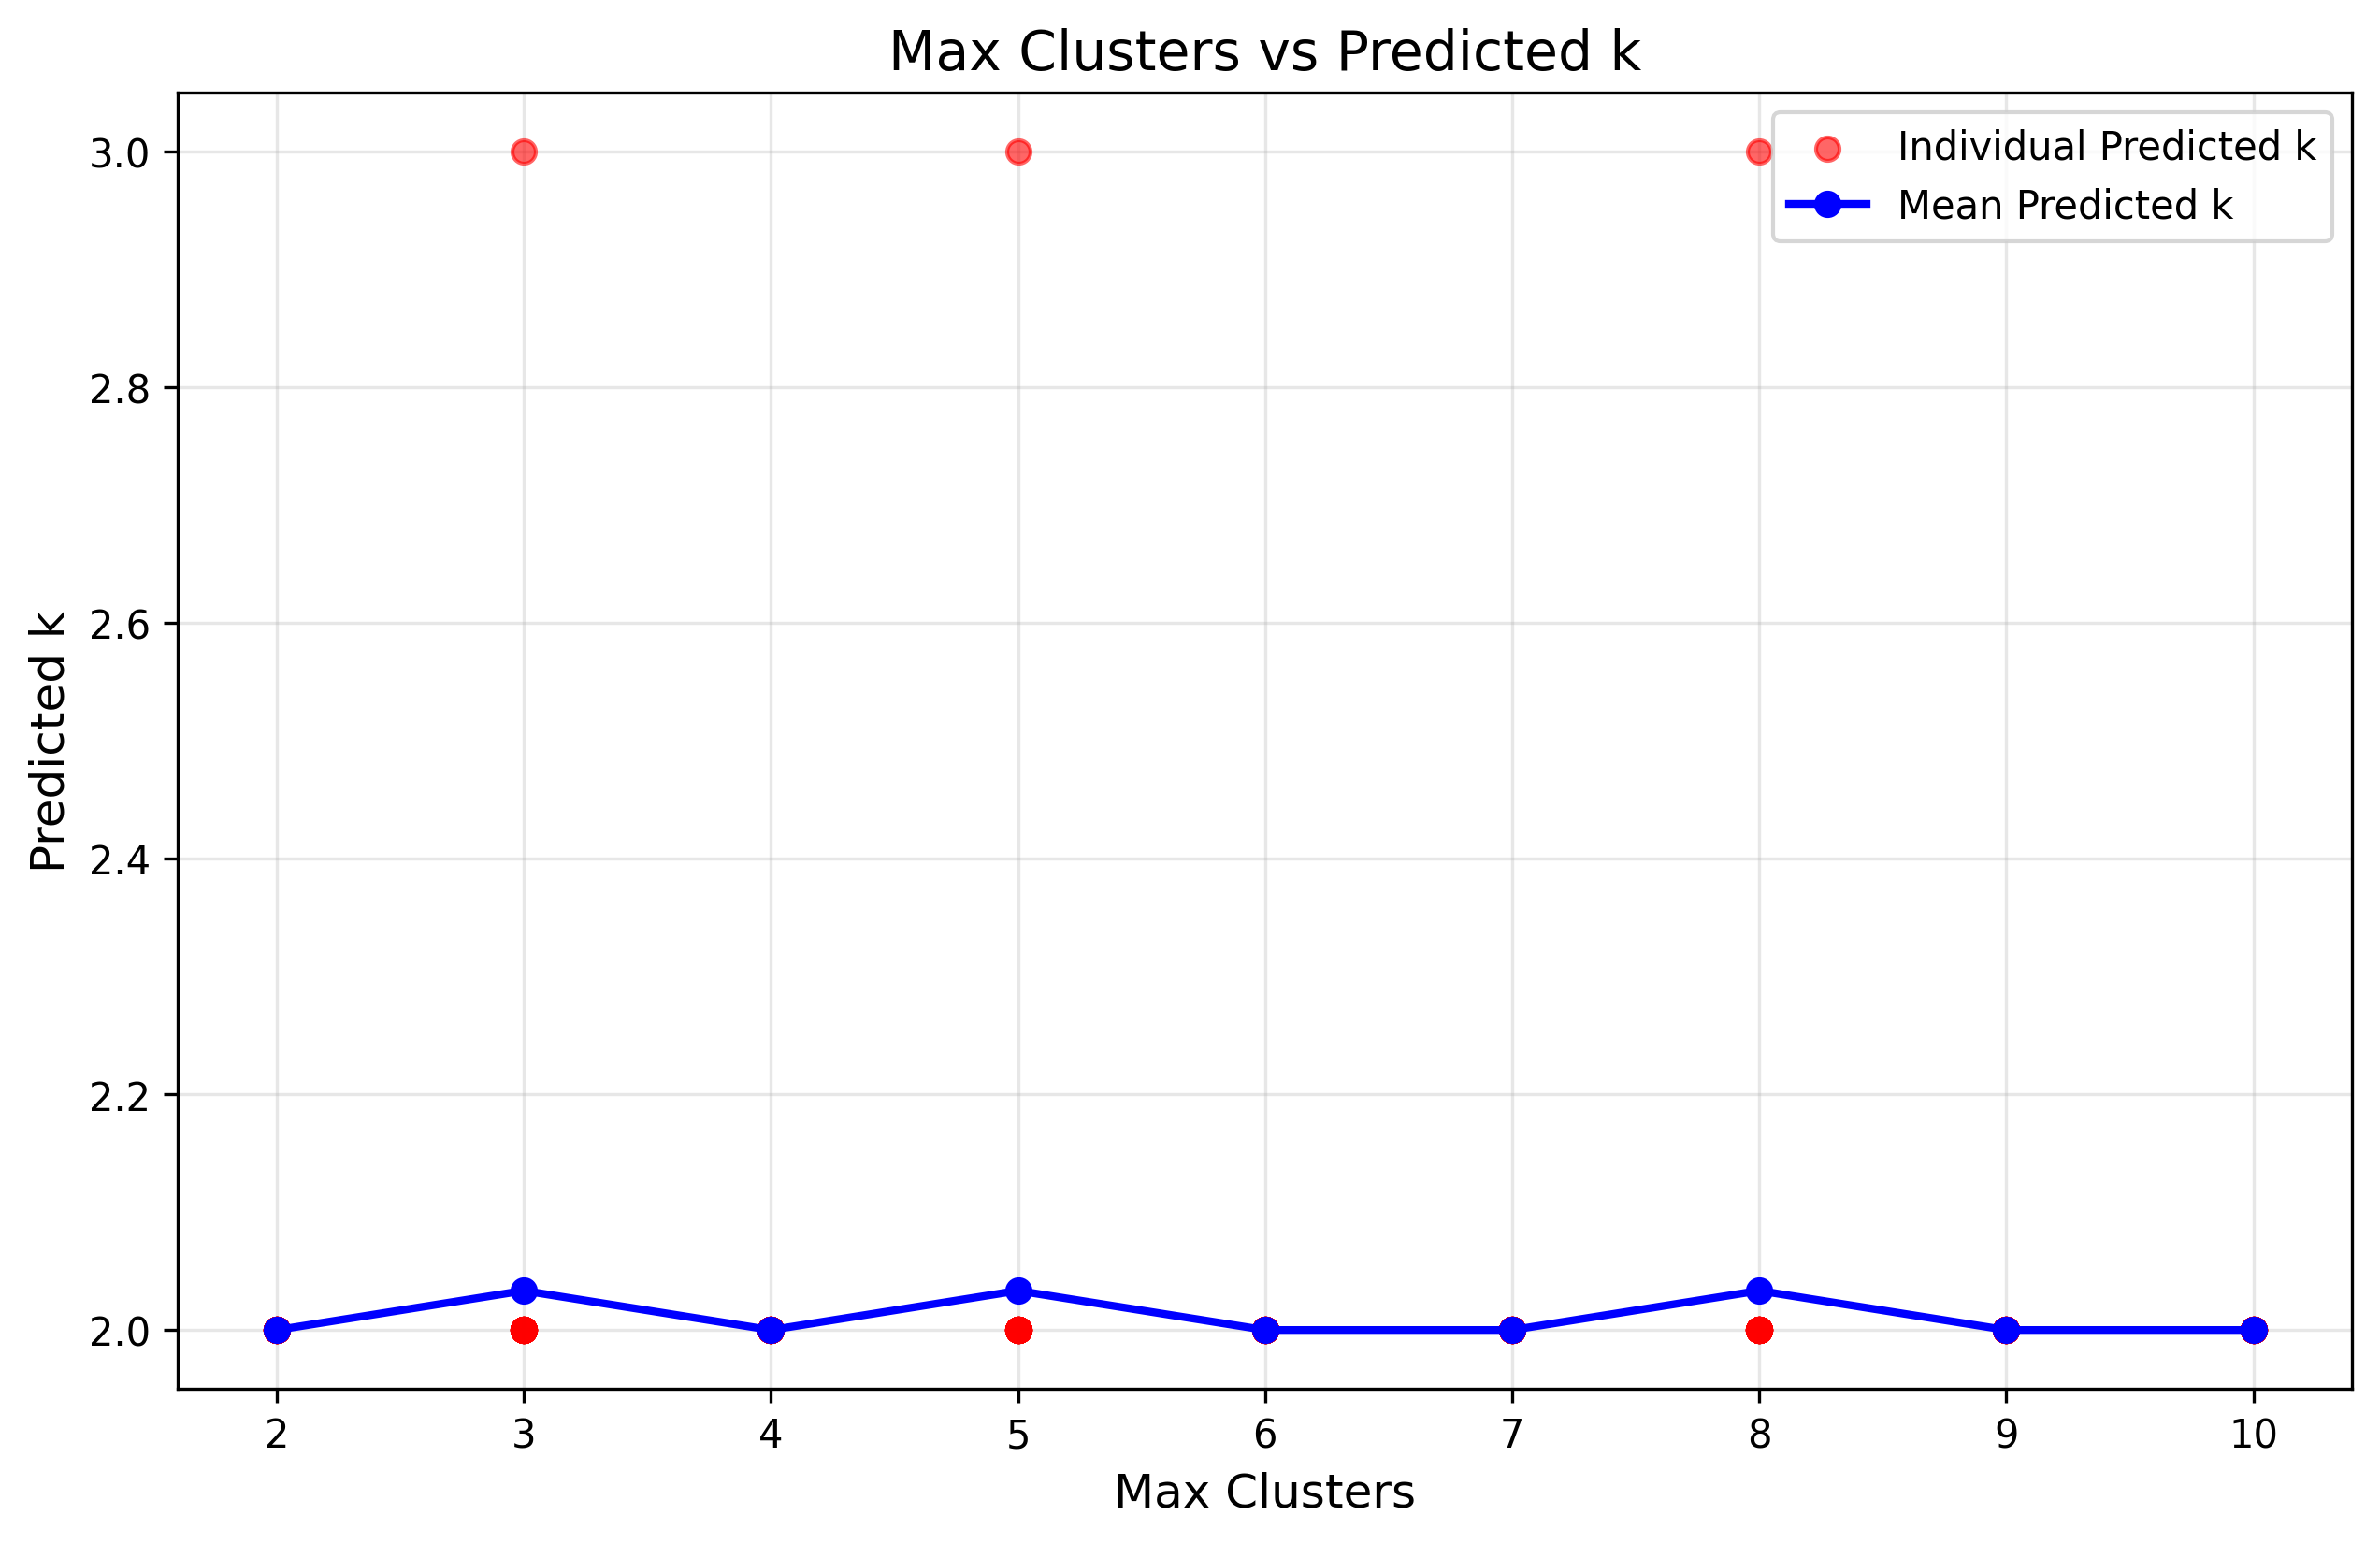
\includegraphics[width=\linewidth]{figures/XMeans/hepatitis_max_k_vs_predicted_k.png}
		\caption{Hepatitis dataset}
		\label{fig:hepatitis_max_k}
	\end{subfigure}
	\begin{subfigure}[b]{0.32\textwidth}
		\centering
		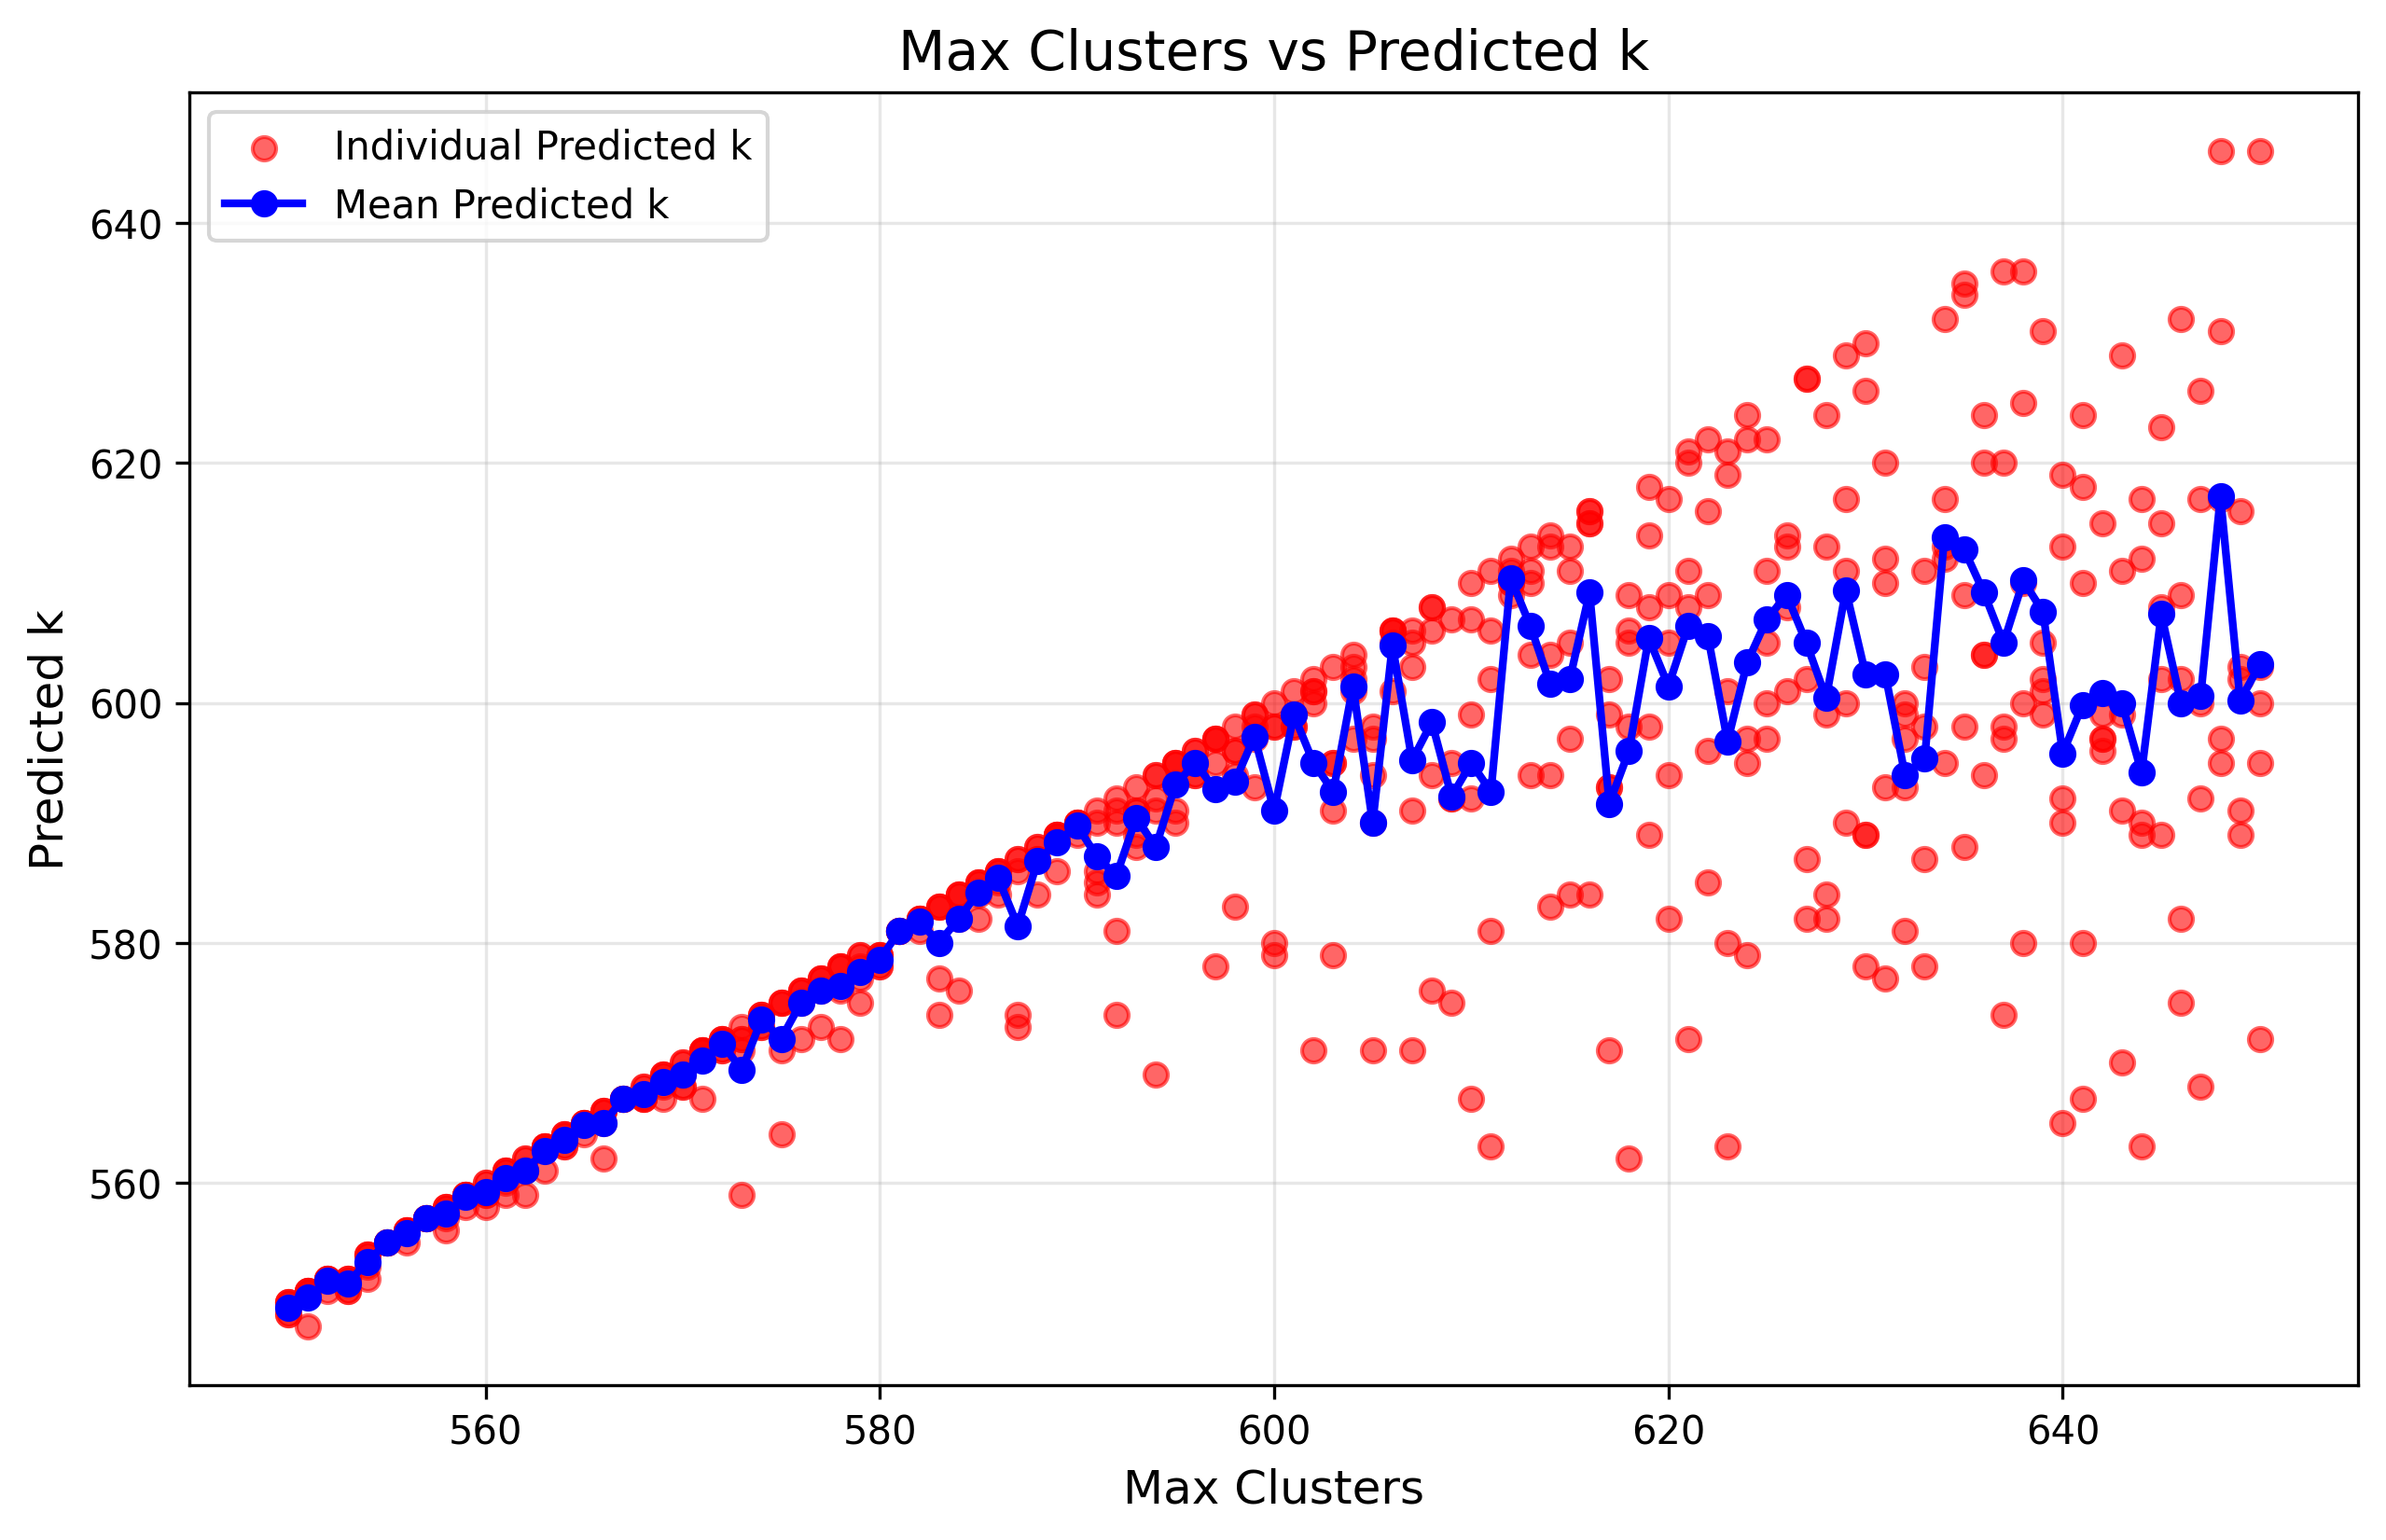
\includegraphics[width=\linewidth]{figures/XMeans/mushroom_max_k_vs_predicted_k.png}
		\caption{Mushroom dataset}
		\label{fig:mushroom_max_k}
	\end{subfigure}
	\begin{subfigure}[b]{0.32\textwidth}
		\centering
		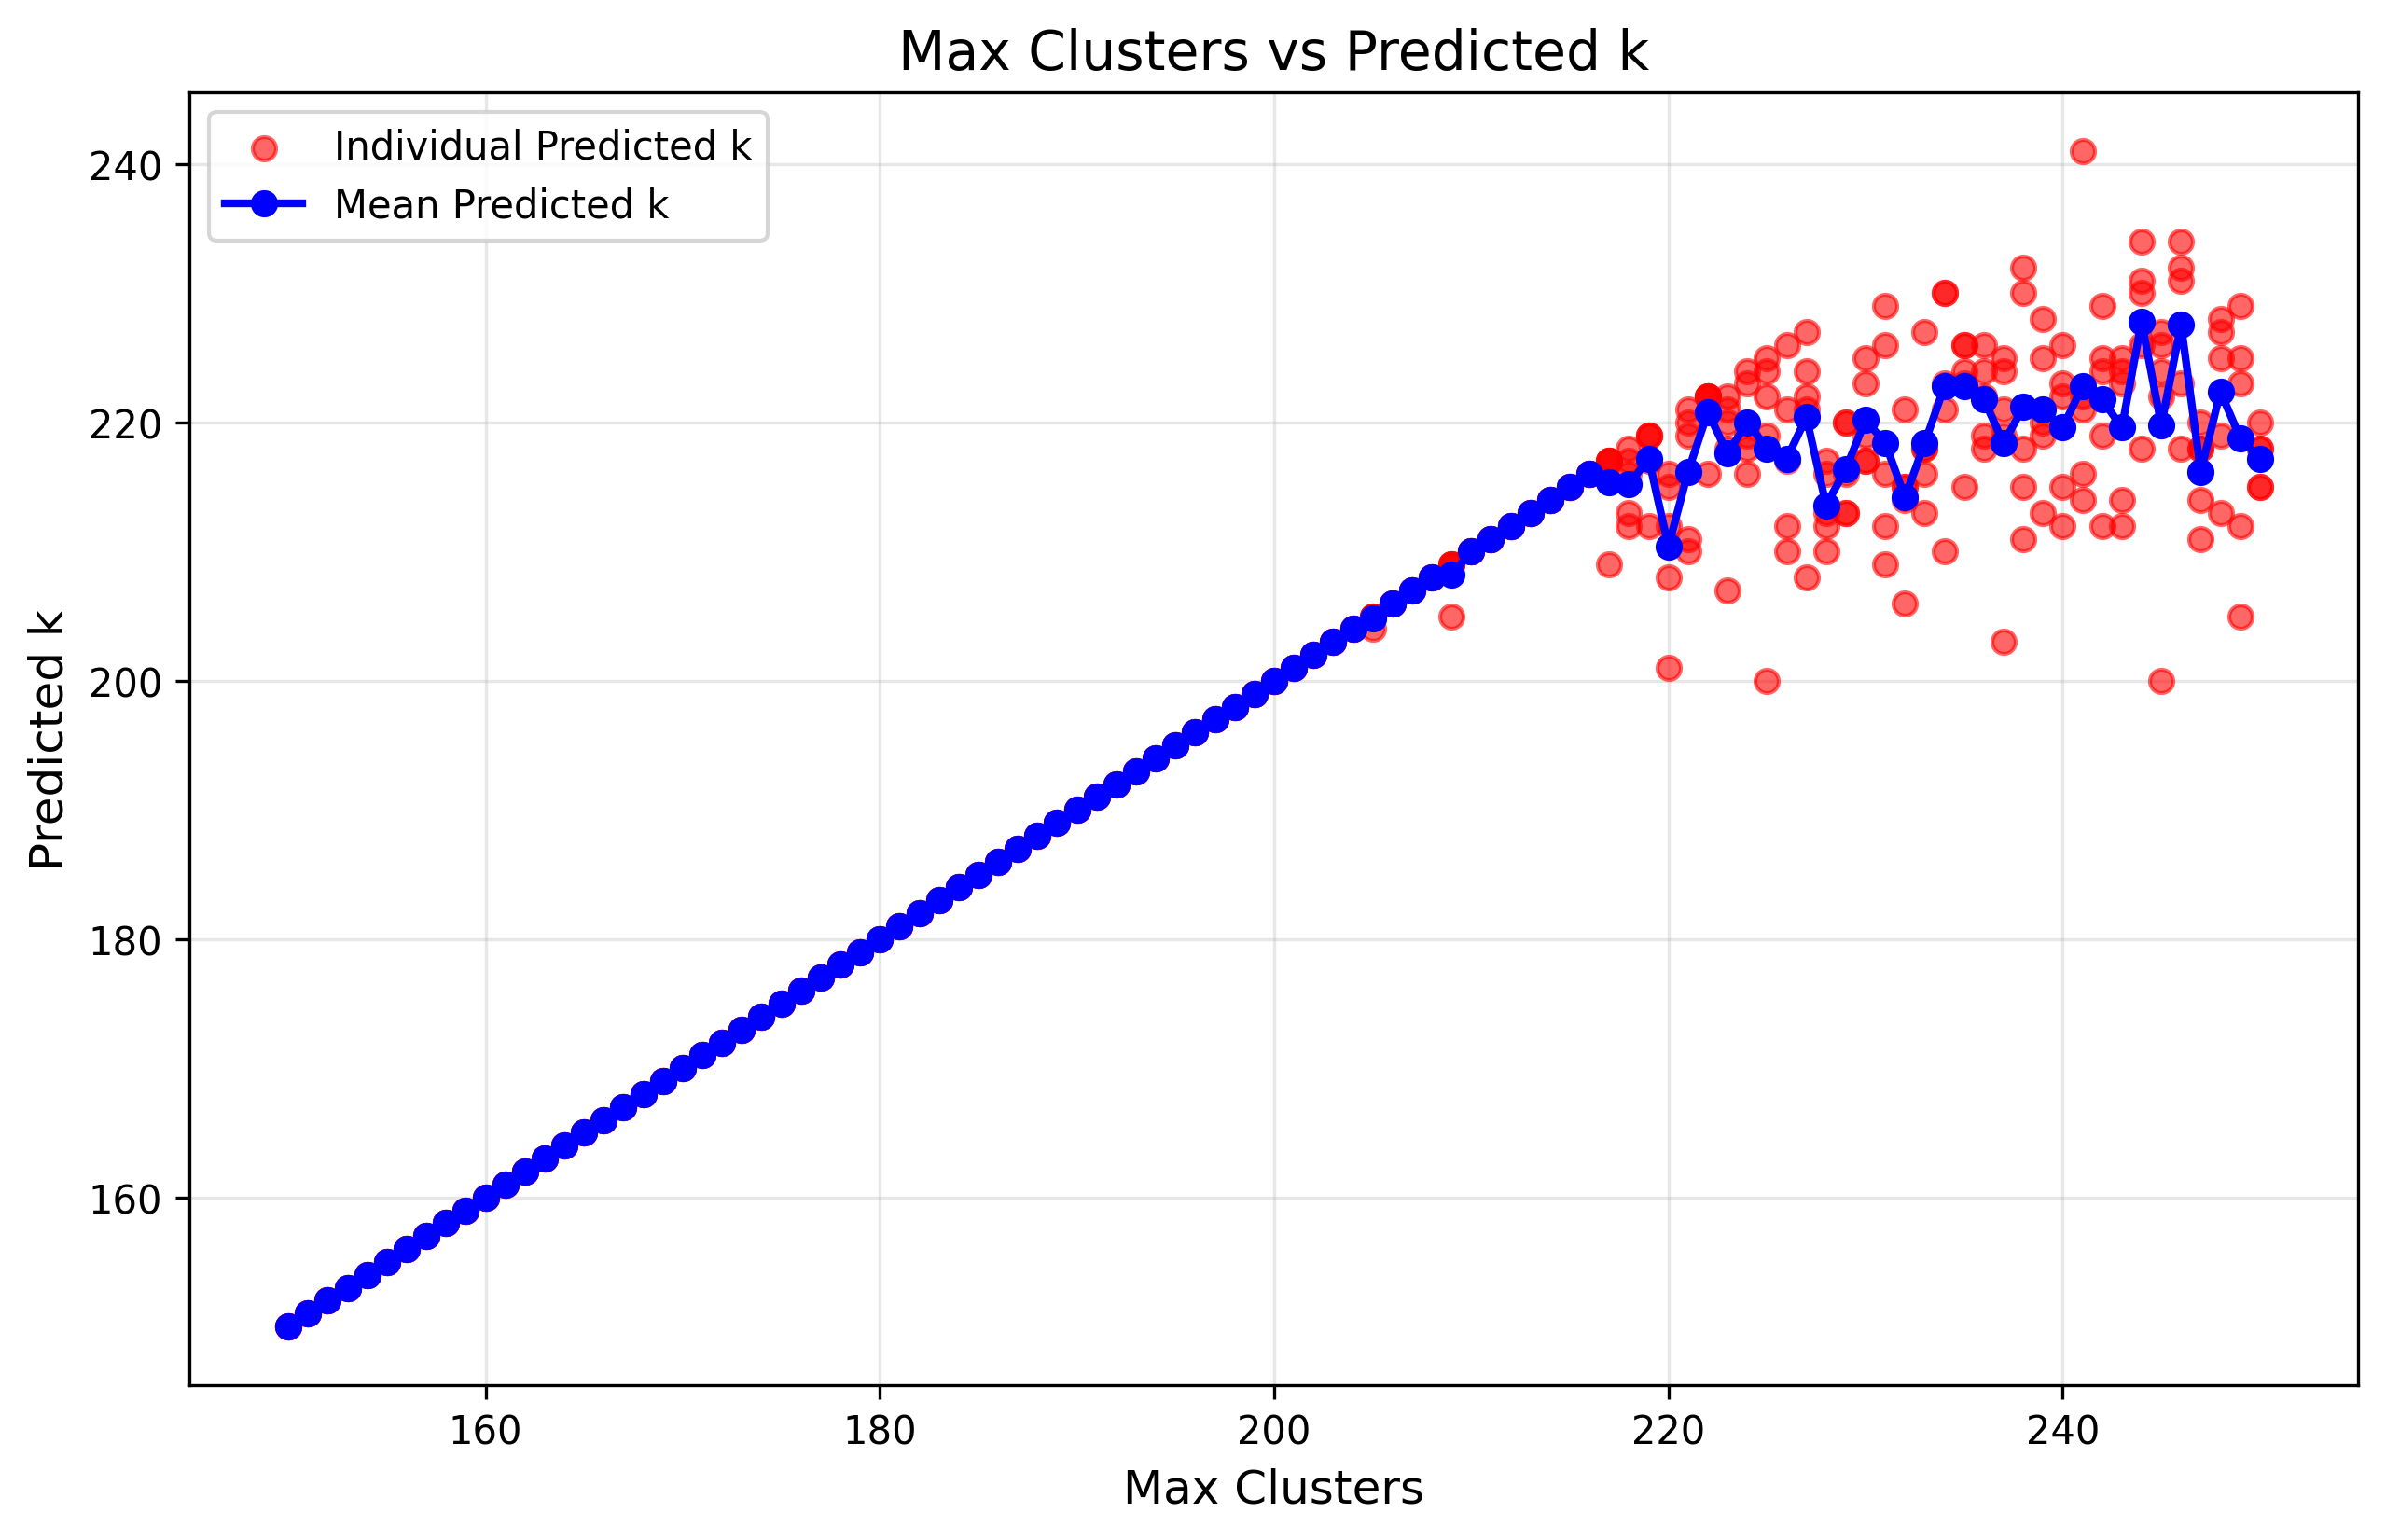
\includegraphics[width=\linewidth]{figures/XMeans/pen-based_max_k_vs_predicted_k.png}
		\caption{Pen-based dataset}
		\label{fig:pen_based_max_k}
	\end{subfigure}
	\caption{Effect of maximum clusters on predicted clusters for different datasets.}
	\label{fig:xmeans_max_clusters}
\end{figure}

\begin{enumerate}
	\item \textbf{Hepatitis:}
	\\ The X-Means algorithm generally converges to 2 clusters. The average predicted clusters remain stable across a range of maximum cluster values from 2 to 10, with rare runs showing 3 clusters.
	
	\item \textbf{Mushroom:}
	\\ For the mushroom dataset, the results are different. Runs with a maximum number of clusters lower than 600 always converged to the maximum. For higher values, the algorithm repeatedly found fewer clusters, particularly noticeable when plotting the average predicted clusters (blue line).
	
	\item \textbf{Pen-based:}
	\\ Similar to the mushroom dataset, the pen-based dataset saw the algorithm converge to a lower number of clusters, around 200 (see Figure~\ref{fig:pen_based_max_k}).
\end{enumerate}

\subsubsection{Visualization}

The datasets' high dimensionality necessitated using Principal Component Analysis (PCA) for visualization. The hepatitis dataset has fewer samples and converges to fewer clusters, allowing for 2D visualization. For the mushroom and pen-based datasets, 3D plots are more informative.

\begin{figure}[H]
	\centering
	\begin{subfigure}[b]{0.32\textwidth}
		\centering
		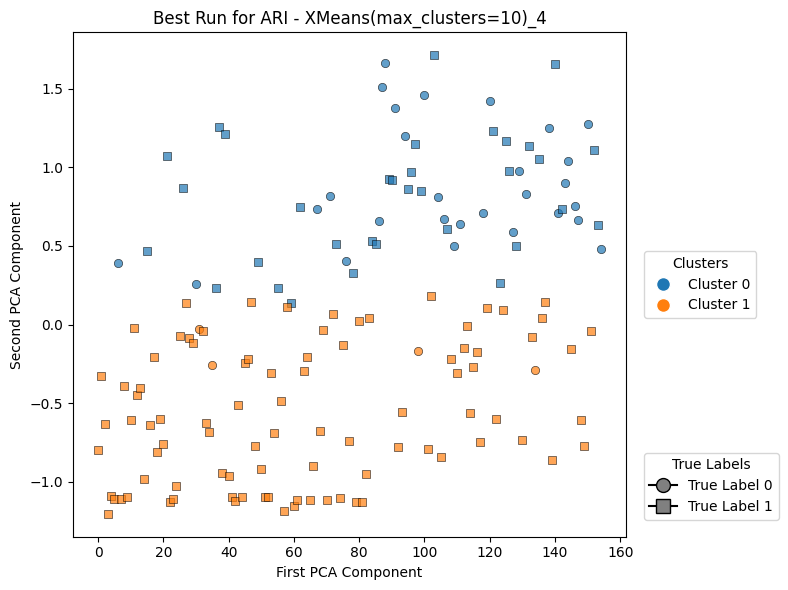
\includegraphics[width=\linewidth]{figures/XMeans/hepatitis_visualization.png}
		\caption{Hepatitis dataset}
		\label{fig:hepatitis_visualization}
	\end{subfigure}
	\begin{subfigure}[b]{0.32\textwidth}
		\centering
		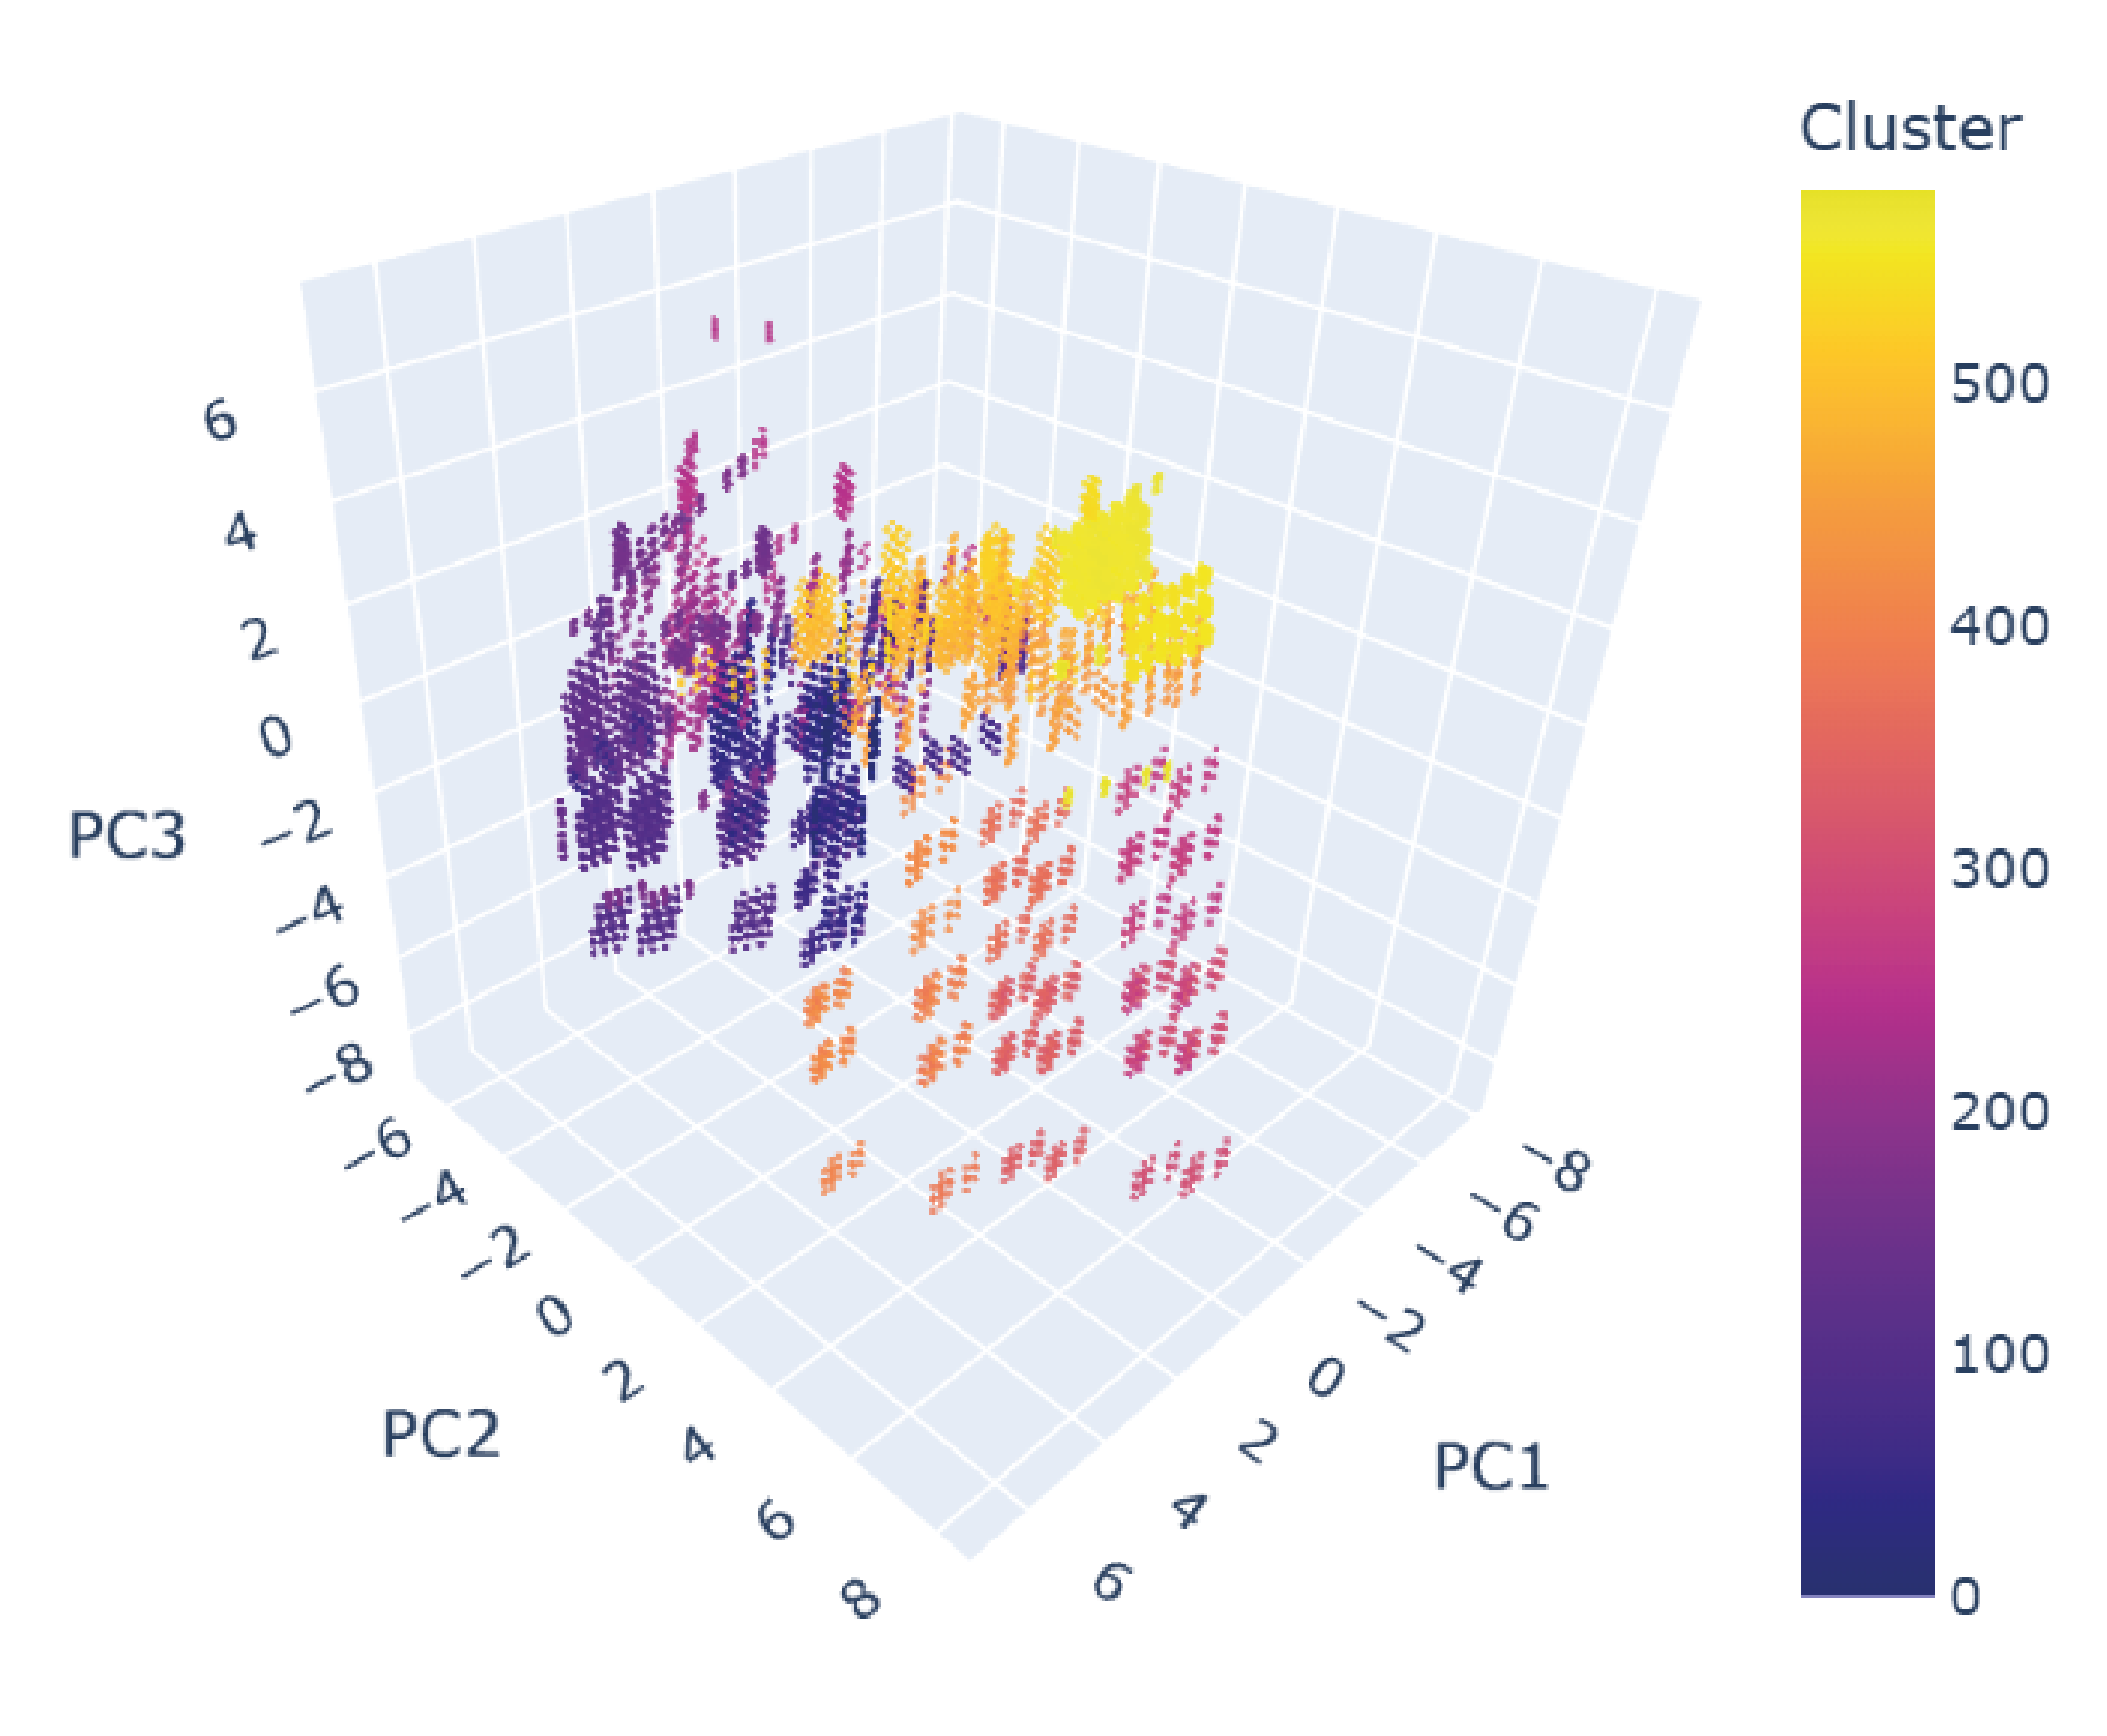
\includegraphics[width=\linewidth]{figures/XMeans/mushroom_visualization.png}
		\caption{Mushroom dataset}
		\label{fig:mushroom_visualization}
	\end{subfigure}
	\begin{subfigure}[b]{0.32\textwidth}
		\centering
		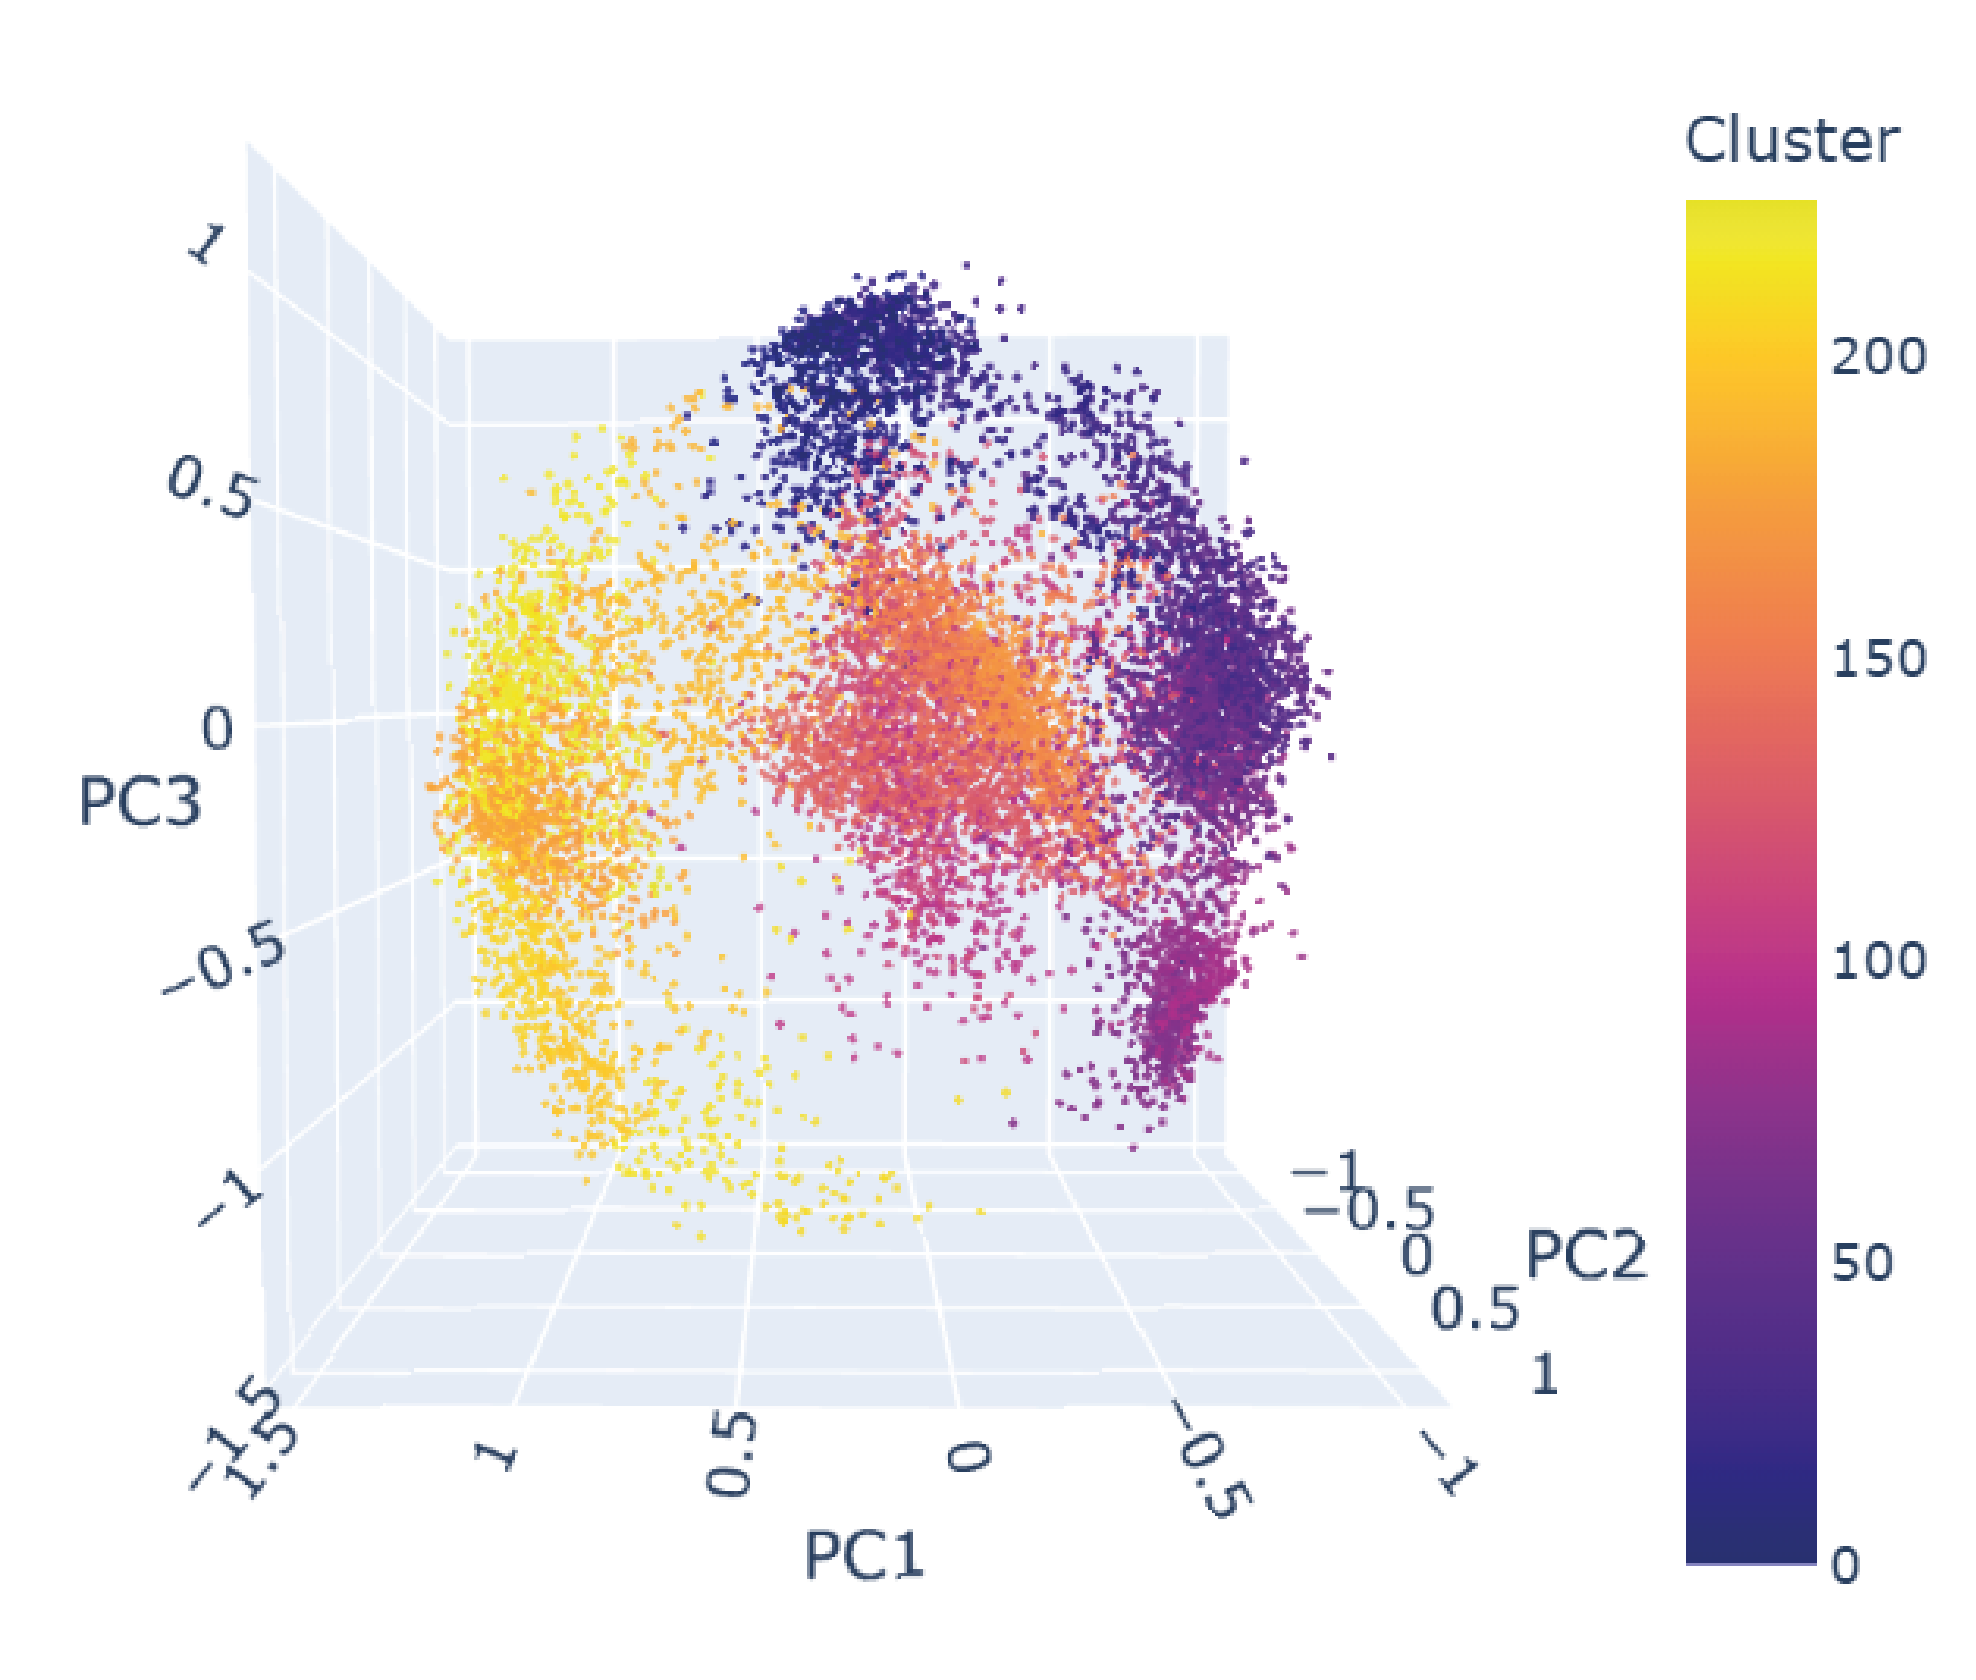
\includegraphics[width=\linewidth]{figures/XMeans/pen-based_visualization.png}
		\caption{Pen-based dataset}
		\label{fig:pen_based_visualization}
	\end{subfigure}
	\caption{Visualization of clusters using PCA.}
	\label{fig:xmeans_visualization}
\end{figure}

\begin{enumerate}
	\item \textbf{Hepatitis:}
	\\ In the 2D plot (Figure~\ref{fig:hepatitis_visualization}), the clusters are clearly divided along the middle.
	
	\item \textbf{Mushroom:}
	\\ The mushroom dataset (Figure~\ref{fig:mushroom_visualization}) shows large elongated clusters that decompose into smaller, well-separated clusters upon closer inspection.
	
	\item \textbf{Pen-based:}
	\\ Similar to the mushroom dataset, the pen-based dataset (Figure~\ref{fig:pen_based_visualization}) reveals that large clusters are composed of smaller, distinct clusters.
\end{enumerate}
